\documentclass[12pt]{article}
\usepackage{geometry}
%\usepackage{times}
\geometry{a4paper, left=1in, right=1in, bottom=1in, top=1in}
\usepackage{authblk}
\usepackage{fancyhdr}
\usepackage{graphicx}
\usepackage{tabularx}

%define vars
\newcommand{\tit}{Intall Abaqus 2017 on a Linux System}
\newcommand{\ifp}{\textit{InstallationFilesRootPath}}

%Title page
\title{
\includegraphics[height=1in]{Figures/NUIG_Logo.jpg}\\ \tit}
\author[1]{Yadong Jiang}
\affil[1]{College of Engineering and Informatics, National University of Ireland Galway}
\date{}




%Header and footer
\pagestyle{fancy}
\fancyhf{}
\lhead{
\includegraphics[height=0.5in]{Figures/NUIG_Logo.jpg}}
%\rhead{Yadong Jiang}
\rhead{\tit}
\setlength{\headsep}{0.5in}
\rfoot{Page \thepage}

%Tabular
\def\arraystretch{1.5}

\begin{document}
\maketitle

\newpage

\section*{Description}

\begin{table}[h!]
    \label{tb-1}
    \caption{Environments of Installation}
    \begin{center}
        \begin{tabular}{l l}
            \hline
            Linux Distribution: & Ubuntu 14.04.4 LTS (64 bits)\\
            \hline
            Linux desktop environment: & N/A \\
            \hline
            Abaqus version: & Abaqus 2017 (64 bits) \\
            \hline
        \end{tabular}
    \end{center}
\end{table}


\section*{Prerequirments}

\subsection*{Install Required Packages}

\subsection{Disguise Ubuntu as CentOS}
\begin{figure}[h!]
\label{fig-1}
\begin{center}
    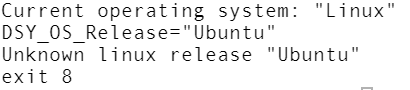
\includegraphics[width=0.5\textwidth]{Figures/UnknowLinux.png}
\end{center}
\caption{Unknown linux release}
\end{figure}


\begin{table}
\label{tb-2}
\caption{Folders which contain the "Linux.sh" files}
\begin{center}
\begin{tabular}{l}
    \hline
    \ifp/1/inst/common/init \\
    \hline
    \ifp/1/SIMULIA\_Documentation/AllOS/1/inst/common/init \\
    \hline
    \ifp/2/SIMULIA\_FLEXnet\_LicenseServer/Linux64/1/inst/common/init \\
    \hline
    \ifp/2/SIMULIA\_AbaqusServices/Linux64/1/inst/common/init \\
    \hline
    \ifp/2/SIMULIA\_AbaqusServices\_CAA\_API/Linux64/1/inst/common/init \\
    \hline
    \ifp/2/SIMULIA\_Abaqus\_CAE/Linux64/1/inst/common/init \\
    \hline
    \ifp/2/SIMULIA\_Tosca/Linux64/1/inst/common/init \\
    \hline
    \ifp/3/SIMULIA\_Isight/Linux64/1/inst/common/init \\
    \hline
\end{tabular}
\end{center}
\end{table}



\section*{Installation}

\section*{Start Abaqus}
\end{document}